\documentclass[14pt,fleqn]{extarticle}
\RequirePackage{prepwell-eng}
\previewoff

\newcommand\ans{\cos^{-1} \frac{1}{\sqrt{3}}}
\newcommand\kexp{ \left(\frac{\pi L^3}{3} \right)}
\newcommand\ea{ \left(3\cos^2\theta-1 \right)}

\begin{document}

\begin{problem}
	\statement 
    
    Show that the semi-vertical angle of the cone with maximum volume and given 
    slant height is $\ans$      
    
    \begin{step}
  \begin{options} 
        
    \end{options} 
     \reason 
     
     The problem statement says that the slant-height $(L)$ is known and that 
     the volume is the maximum possible \newline 
     
     Hence, our objective is as follows 
     \begin{center}
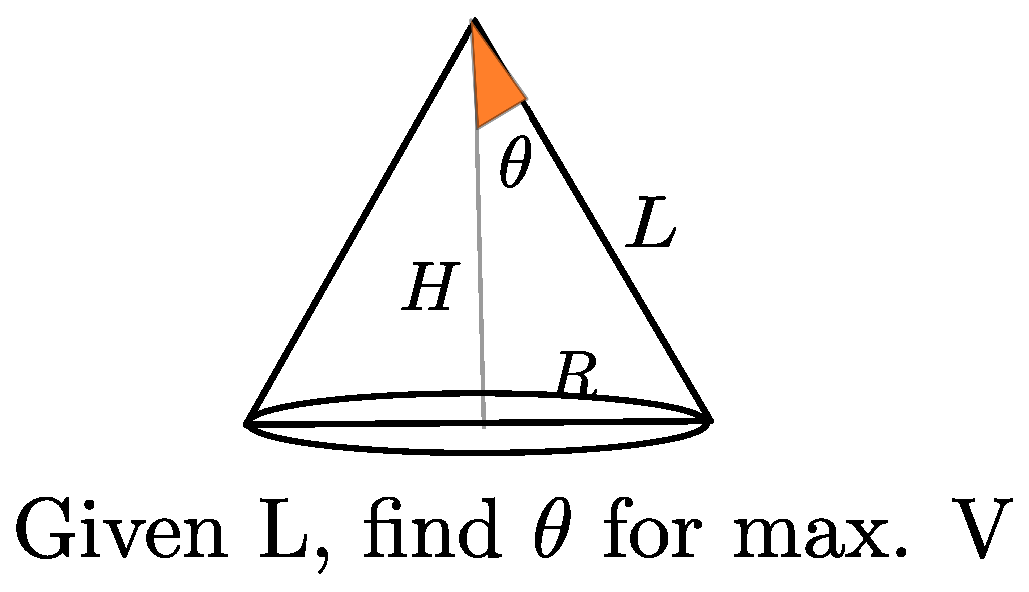
\includegraphics[scale=0.45]{figure.eps}
\end{center}
\end{step}


\begin{step}
  \begin{options} 
     \correct 
     \[ \qquad V = \kexp \sin^2\theta\cdot \cos\theta \]  
     \incorrect
        \[ \qquad V = \kexp \sin\theta\cdot \cos^2\theta \]
    \end{options} 
     \reason 
       
     Referring to the figure from before 
     \[ \qquad R = L\sin\theta \text{ and } H = L\cos\theta \] 
     And hence, 
     \begin{align}
	V &= \frac{1}{3}\pi R^2 H = \frac{1}{3}\pi \left(L\sin\theta \right)^2\cdot \left( L\cos\theta \right) \\
	&= \kexp \sin^2\theta\cdot \cos\theta 
\end{align}
\end{step}

\begin{step}
  \begin{options} 
     \correct 
       \begin{align}
	V' &= \kexp\cdot\cos\theta\cdot \left(3\cos^2\theta - 1 \right)
\end{align}

     Which means, $V$ has extreme values at \[\qquad \theta = 0\text{ and } \theta = \ans\]
     \incorrect
     
     \begin{align}
	V' &= \kexp\cdot\sin\theta\cdot \left(3\cos^2\theta - 1 \right)
\end{align}

     Which means, $V$ has extreme values at \[\qquad \theta = \frac{\pi}{2}\text{ and } \theta = \ans\]
        
    \end{options} 
     \reason 
     
     \begin{align}
	V &= \kexp \sin^2\theta\cdot\cos\theta \\
	\therefore \frac{dV}{d\theta} &= V' = \underbrace{\kexp \left[2\sin\theta\cos^2\theta - \sin^3\theta \right]}_{\text{Product Rule}} \\
	&= \kexp\cdot\sin\theta \left(2\cos^2\theta-\sin^2\theta \right) \\
	&= \kexp \cdot\sin\theta\cdot \underbrace{\left(3\cos^2\theta - 1 \right)}_{\sin^2\theta = 1 - \cos^2\theta} \\
	\text{So } V' &= 0 \implies \sin\theta = 0\text{ or } \cos\theta = \frac{1}{\sqrt{3}} \\
	\text{or } \theta &= \sin^{-1} 0 = 0\text{ and }\theta = \cos^{-1} \frac{1}{\sqrt{3}}
\end{align}

       Hence, the \underline{extremas} occur when \[ \qquad \theta=0\text{ and } \theta = \cos^{-1} \frac{1}{\sqrt{3}} \]
\end{step}

\begin{step}
  \begin{options} 
     \correct 
       
       \begin{center}
  \begin{tabular}{NNNc}
   \toprule
       \theta & V' & V'' & Meaning  \\
   \midrule 
   0 & 0 & 2\kexp & Minima \\
    \midrule 
    \cos^{-1} \frac{1}{\sqrt{3}} & 0 & -\frac{2\sqrt{2}}{\sqrt{3}}\kexp & Maxima \\
    \bottomrule
  \end{tabular}
\end{center}
Hence, $V$ is maximum when $\theta = \cos^{-1} \frac{1}{\sqrt{3}}$ 

     \incorrect
     
     
       \begin{center}
  \begin{tabular}{NNNc}
   \toprule
       \theta & V' & V'' & Meaning  \\
   \midrule 
   0 & 0 & \kexp & Minima \\
    \midrule 
    \cos^{-1} \frac{1}{\sqrt{3}} & 0 & -\frac{2}{3}\kexp & Maxima \\
    \bottomrule
  \end{tabular}
\end{center}
Hence, $V$ is maximum when $\theta = \cos^{-1} \frac{1}{\sqrt{3}}$ 

    \end{options} 
     \reason 
     
     Common sense says that 
     \[ \qquad V \geq 0 \text{ and } V\to 0\text{ as }\theta\to 0 \]
     Hence, the minimum volume the cone can have is $0$ at $\theta = 0$ \newline 
     
     And therefore, at the other $\theta$ for which $V\neq 0$ must be the maxima \newline 
     
     Nevertheless, if you want to be dead sure, then find $V''$ 
     
     \smallmath
     \begin{align}
	    &V' = \kexp\sin\theta\cdot \left(3\cos^2\theta -1 \right) \\
	    \therefore &V'' = \frac{d}{d\theta}V' = \kexp \frac{d}{d\theta} \left[\sin\theta\cdot (3\cos^2\theta -1) \right] \\
	    &= \kexp \underbrace{\left[ \ea\cdot \cos\theta + \sin\theta\cdot \left(-6\cos\theta\sin\theta \right)\right]}_{\text{Product Rule}}\\
	    &= \kexp \cos\theta\cdot\left(3\cos^2\theta-6\cos\theta\sin\theta-1 \right) \\
	    &= 2\kexp > 0 \text{ for } \theta = 0 \\
	    &= \underbrace{-\frac{2\sqrt{2}}{\sqrt{3}}\kexp < 0 \text{ for } \theta = \cos^{-1} \frac{1}{\sqrt{3}}}_{\cos\theta = \frac{1}{\sqrt{3}} \implies \sin\theta = \sqrt{1- \frac{1}{3}} = \sqrt{\frac{2}{3}}}
\end{align}
       
\end{step}
\end{problem} 

\end{document}